\subsection{CFDBench (Fluid Dynamics)}
{{\footnotesize
\noindent CFDBench provides large-scale CFD data for four canonical fluid flow problems, 
assessing neural operators' ability to generalize to unseen PDE parameters and domains.


\begin{description}[labelwidth=4cm, labelsep=1em, leftmargin=4cm, itemsep=0.1em, parsep=0em]
  \item[date:] 2024-10-01
  \item[version:] 1
  \item[last\_updated:] 2024-10-01
  \item[expired:] false
  \item[valid:] yes
  \item[valid\_date:] 2024-10-01
  \item[url:] \href{https://arxiv.org/abs/2310.05963}{https://arxiv.org/abs/2310.05963}
  \item[doi:] 10.48550/arXiv.2310.05963
  \item[domain:] Fluid Dynamics; Scientific ML
  \item[focus:] Neural operator surrogate modeling
  \item[keywords:]
    - neural operators
    - CFD
    - FNO
    - DeepONet
  \item[licensing:] CC-BY-4.0
  \item[task\_types:]
    - Surrogate modeling
  \item[ai\_capability\_measured:]
    - Generalization of neural operators for PDEs
  \item[metrics:]
    - L2 error
    - MAE
  \item[models:]
    - FNO
    - DeepONet
    - U-Net
  \item[ml\_motif:]
    - Generalization
  \item[type:] Benchmark
  \item[ml\_task:]
    - Supervised Learning
  \item[solutions:] Numerous, as it's a benchmark for ML models
  \item[notes:] 302K frames across 739 cases
  \item[contact.name:] Yining Luo
  \item[contact.email:] yining.luo@mail.utoronto.ca
  \item[datasets.links.name:] unknown
  \item[datasets.links.url:] \href{unknown}{unknown}
  \item[results.links.name:] unknown
  \item[results.links.url:] \href{unknown}{unknown}
  \item[fair.reproducible:] True
  \item[fair.benchmark\_ready:] True
  \item[id:] cfdbench\_fluid\_dynamics
  \item[Citations:] \cite{luo2024cfdbenchlargescalebenchmarkmachine}
\end{description}

{\bf Ratings:} ~ \\

\begin{tabular}{p{0.15\textwidth} p{0.07\textwidth} p{0.7\textwidth}}
\hline
Rating & Value & Reason \\
\hline
dataset & 0 & Not given
 \\
documentation & 5 & Associated paper gives all necessary information.
 \\
metrics & 5 & Quantitative metrics (L2 error, MAE, relative error) are clearly defined and align with regression task objectives.
 \\
reference\_solution & 5 & Baseline models like FNO and DeepONet are implemented, hardware specified.
 \\
software & 5 & The benchmark provides Python scripts for data loading, preprocessing, and model training/evaluation
 \\
specification & 0 & Not listed
 \\
\hline
\end{tabular}

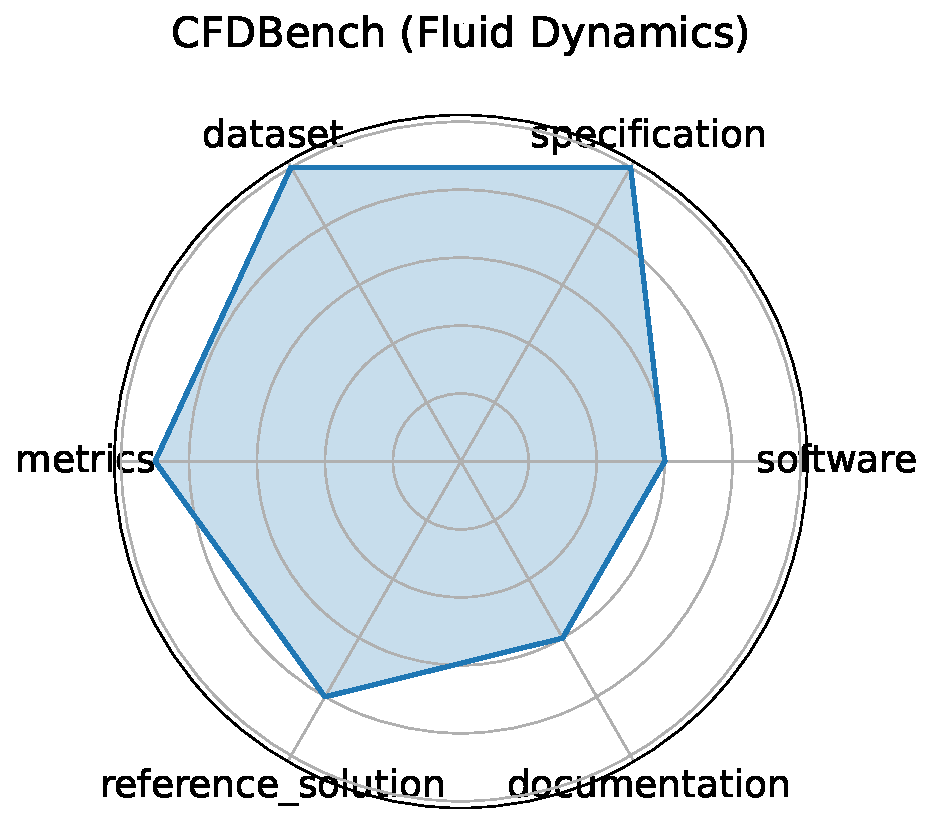
\includegraphics[width=0.2\textwidth]{cfdbench_fluid_dynamics_radar.pdf}
}}
\clearpage